\chapter{On Fidelity per Unit Cost}\label{ch:fidelity}

While the previous chapter was about concrete communication schemes for the
Gaussian channel, we return in this chapter to more general sources and
channels.  We consider three standard communication problems, namely source
coding with a fidelity criterion, channel coding  with a channel input
constraint, and the combined problem of reproducing a source across a noisy
channel. Our focus here is on discrete memoryless sources and channels, but the
essence of our results extends to continous alphabets. 

We begin by addressing the channel coding problem in Section~\ref{sec:cuc}. We
consider the capacity per unit cost, a concept that is traceable in various
forms as far back as Reza~\cite{Reza1961} (see also references
in~\cite{Verdu1990}) and was more recently studied by Gallager
(\cite{Gallager1988}, \cite[Ch.~14]{BlahutK2002}) and developed by Verd\'u in
his influential paper~\cite{Verdu1990} (see also~\cite{Verdu2002}).

The capacity per unit cost for a channel with transition probabilities~$\pyx$
and input cost measure~$\rho(x)$ is defined as \[ \Ch = \sup_{\px}
\frac{I(X;Y)}{\E[\rho(X)]}, \] where the supremum is taken over all possible
input distributions~$\px$.  Usually $\pyx$ and $\rho(x)$ are given, and to
compute the capacity per unit cost one maximizes over the space of input
distributions. For the case when a channel input symbol of zero cost exists,
however, Verd\'u showed that the capacity per unit cost can be obtained by a
simpler maximization over the channel input alphabet.

We look at the problem from a different angle. We show that for fixed $\px$ and
$\pyx$ there is a simple expression for the cost measure~$\rho(x)$ for which
$\px$ achieves the capacity per unit cost. This criterion is applicable whether
or not a zero-cost symbol exists; it follows from refining a similar criterion
that Gastpar et al.~\cite{GastparRV2003} developed for the purpose of achieving
capacity rather than capacity per unit cost.

We illustrate our result with a detailed example of a Gaussian channel with
Gaussian input.  First we find that the cost measure for which the system
operates at capacity per unit cost is of the form $\rho(x) = x^2 + k$ for some
positive constant~$k$ (to be specified). We show that a discrete-time channel
with this cost measure relates to a continuous-time channel for which power can
be traded against bandwidth.  Furthermore, the tradeoff that maximizes the rate
(in bits\slash second) of the continuous-time channel corresponds to the
operating point at which the discrete-time channel achieves the capacity per
unit cost.

For the rate-distortion problem a similar result exists, which we explore in
Section~\ref{sec:rddual}. For reasons that will become apparent, it is more
convenient to study this result in terms of a fidelity measure, defined as the
negative of the distortion measure. Following this line of
thought we define the \emph{fidelity per unit rate} of a source:
it is to source coding what the capacity per unit cost is to channel coding.
Again refining a result by Gaspar et al., we give a condition for a test
channel\footnote{In rate-distortion theory, a test channel is a conditional
distribution of the reconstruction given a source symbol.}
to achieve the fidelity per unit rate of the source. 

In Section~\ref{sec:fidcostbound} we consider the end-to-end problem of
reproducing a source across a noisy channel. Drawing on the results of
Sections~\ref{sec:cuc} and~\ref{sec:rddual}, we show that the capacity per unit
cost and the fidelity per unit rate can be combined to give the \emph{fidelity
per unit cost}, \ie, the maximum ratio of fidelity per cost at which a
source-channel coding system can operate.

The set of communication systems that operate at fidelity per unit cost is a
subset of the set of communication systems that are optimal in the sense of
\defref{optimality} of \chapref{fundamentals} (page~\pageref{def:optimality}).
In the last result of the present chapter we give necessary and sufficient
conditions under which a given communication  system operates at fidelity per
unit cost. This can be seen in analogy to \thmref{optimalityconditions}, which
gave necessary and sufficient conditions for a communication system to be
optimal according to \defref{optimality}.


\section{Achieving Capacity per Unit Cost}
\label{sec:cuc}

Let $\pyx$ be the transition distribution of a discrete memoryless channel and
let $\px$ and $\qx$ be two arbitrary but fixed input distributions. Let $\py$
and $\qy$ be the corresponding output distributions, \ie, 
\begin{align*}
  \py(y) &= \sum_x \px(x) \pyx(y|x) \quad\text{and} \\
  \qy(y) &= \sum_x \qx(x) \pyx(y|x).
\end{align*}
Define $\ro(x)$ through $\px$ as
\begin{equation}
  \label{eq:optrho}
  \ro(x) = \DD.
\end{equation}
Let $\E_P$ and $\E_Q$ denote expectations with respect to $\px$ and $\qx$,
respectively, and let $I_P(X;Y)$ and $I_Q(X;Y)$ denote the mutual informations
corresponding to these input distributions. 

\begin{proposition}
  \label{prop:ratepercost}
  We have
  \begin{equation}
    \label{eq:ratepercost}
    \frac{\Iq(X;Y)}{\Expq[\ro(X)]} \le \frac{\Ip(X;Y)}{\Ep[\ro(X)]} = 1,
  \end{equation}
  with equality if and only if $Q_X = P_X$.
\end{proposition}

Proposition~\ref{prop:ratepercost} implies that if the channel input cost
function is as in~\eqref{eq:optrho} (up to scaling), then $P_X$ achieves the
capacity per unit cost.

\begin{proof}
  First note that $\Ep[\ro(X)] = \Ip(X;Y)$, \ie, $\Ip(X;Y) / \Ep[\ro(X)] = 1$.
  On the other hand, if the input distribution is $\qx$ then
  \begin{align*}
    \lefteqn{\Expq[\ro(X)] - \Iq(X;Y)} \\
%    &=
%    \sum_x \qx(x) \DD - \sum_{x,y} \qx(x) \pyx(y|x) \log
%    \frac{\pyx(y|x)}{\qy(y)}
%    \\
    &= \sum_{x,y} \qx(x) \pyx(y|x) \left[ \log \frac{\pyx(y|x)}{\py(y)} -
    \log \frac{\pyx(y|x)}{\qy(y)} \right] \\
    &= D(\qy \| \py) \ge 0.
  \end{align*}
  It follows that
  \[ \frac{\Iq(X;Y)}{\Expq [\ro(X)]} \le 1
  \]
  with equality if and only if $P_Y = Q_Y$, or $P_X = Q_X$.
\end{proof}

\begin{remark}
  \label{rem:continuouscuc}
  The proposition also holds for channels with continuous alphabets. This
  follows directly if the sums in the proof are replaced by integrals.
\end{remark}

\begin{example}[BSC]
  \label{ex:bsccap}
  Consider a binary symmetric channel with crossover
  probability~$\epsilon=0.1$. Let the input distribution be such that $\px(0) =
  0.7$ and $\px(1) = 0.3$. Evaluating $\ro(x)$ for this situation yields
  \begin{equation*}
    \ro(0) \approx 0.23 \quad\text{and} \quad
    \ro(1) \approx 0.99.
  \end{equation*}
  The corresponding capacity curve is plotted in \figref{bsccap}.
\end{example}

\begin{example}[Gaussian]
  \label{ex:gausscap}
  Consider the AWGN channel $Y=X+Z$, where $X \sim \N(0,\sxq)$ and $Z \sim
  \N(0,1)$. Evaluating $\ro(x)$, we obtain
  \[ \ro(x) = \DD = ax^2 + b, \]
  where
  \[ a = \frac{1}{2 \ln2 (1+\sxq)} \]
  and
  \[ b = \frac12 \left( \log_2(1+\sxq) - \frac{1}{\ln2} +
  \frac{1}{\ln 2 (1+\sxq)} \right). \]
  The cost constraint $\E[\ro(x)] \le P$ can be written as $\E[X^2] \le
  \frac{P-b}{a}$, so the corresponding capacity-cost function is
  \[ C(P) = \frac12 \log_2 (1 + \frac{P-b}{a}), \quad P \ge b. \]
  It is plotted in Figure~\ref{fig:gausscap}.
\end{example}

\begin{figure}
  \centerline{%
  \subfloat[BSC]{\label{fig:bsccap}\input{figures/bsccuc.tex_t}}%
  \hfil%
  \subfloat[Gaussian]{\label{fig:gausscap}\input{figures/gausscap.tex_t}}%
  }% end \centerline
  \caption{Capacity curves for Examples~\ref{ex:bsccap} (left)
  and~\ref{ex:gausscap} (right). The optimal cost function is such that a
  tangent through the origin touches the the curve in the operating point
  that corresponds to the given input distribution~$\px$.}
\end{figure}

When does a cost measure of the form $\rho(x) = x^2 + b$ make sense? The
following example gives an answer to this question. 

\begin{example}
Consider the problem of designing a communication system that maximizes the
communication rate across a continuous-time Gaussian channel. We are free to
trade bandwidth for power, provided that  $P+k B \leq A$ where $B$ is the
(two-sided) bandwidth, $P$ is the power, and $k$ and $A$ are positive constants.
Using the sampling theorem at intervals of length $T$, $BT=1$, we translate the
above problem into its discrete-time equivalent. To do so we first rewrite the
constraint as $\frac{1}{T} \int_0^T \E[X^2(t)] dt \leq A- k B$ and use the fact
that the discrete-time equivalent of the integral is $\E [X^2]$. Hence the
discrete-time constraint becomes  $\frac{1}{T}\E [X^2] \leq A- \frac{k}{T}$ or,
equivalently, $\E [X^2 + k] \leq AT$. 


With this constraint, the maximum rate at which we can transmit reliably (in
bits/second) is
\[ \frac{C(AT)}{T} = A \frac{C(AT)}{AT} \le A \Ch, \]
where $\Ch$ is the capacity per unit cost of the discrete-time channel. Notice
that we can choose to operate at capacity per unit cost by choosing $T$ such
that   $\frac{C(AT)}{AT}$ achieves the maximum. This implies the optimal
power--bandwidth tradeoff.
\end{example}

\begin{example}[Exponential]\label{ex:expchannel}
  Consider an additive exponential noise channel with nonnegative input
  alphabet $Y = X + N$, where $N$ is exponential with mean $b$. Let the input
  distribution $\px$ be equal to $0$ with probability $\frac{b}{a+b}$ and
  exponentially distributed with mean $a + b$ conditioned on it being positive,
  i.e.,
  \begin{equation}
    \label{eq:extexpinp1}
    \Pr[X = 0] = \frac{b}{a+b}
  \end{equation}
  and
  \begin{equation}
    \label{eq:extexpinp2}
    \Pr[X > x | X > 0] = e^{-x / (a+b)} \;.
  \end{equation}
  Then the input $X$ has mean $a$, and the output $Y$ is exponential with mean
  $a+b$, as shown by Verd\'u in~\cite{Verdu1996}. 

  Drawing further on results from \cite{Verdu1996} we have
  \begin{eqnarray*}
    \ro(x) &=&  \DD \nonumber\\
    &=& \log_2(1 + \frac{a}{b}) + \frac{x - a}{a + b} \log_2 e
  \end{eqnarray*}
  and
  \begin{eqnarray}
    \label{eq:expi}
    I(X;Y) &=& \E[ \DDX] \nonumber\\
    &=& \log_2(1 + \frac{a}{b}) \;.
  \end{eqnarray}
  Solving the cost constraint $\E[\ro(X)] \le P$ for $\E[X]$ then yields
  \begin{equation}
    \label{eq:expconstr}
    \E[X] \le \frac{a + b}{\log_2 e} (P - \log_2 (1 + \frac{a}{b})) + a \;.
  \end{equation}

  For a constraint on the mean, an input distribution in the form of
  \eqref{eq:extexpinp1} and \eqref{eq:extexpinp2} (with corresponding mean $a$)
  achieves capacity on the exponential channel. We can thus replace $a$
  in \eqref{eq:expi} by the right hand side of \eqref{eq:expconstr} to obtain
  the cost-constrained capacity
  \begin{equation}
    \label{eq:ccapexp}
    C(P) = \log_2 \left(1 + \frac{\frac{a+b}{\log_2 e}(P - \log_2(1 +
    a/b)) + a}{b}
    \right).
  \end{equation}
  The corresponding capacity curve is displayed in \figref{expchannel}.
\end{example}

\begin{figure}
  \begin{center}
    \input{figures/expchannel.tex_t}
  \end{center}
  \caption{Capacity curve for the exponential channel of \exref{expchannel}.}
  \label{fig:expchannel}
\end{figure}

%In~\cite{Verdu90} it was shown that if the cost measure is such that there
%exists a symbol of zero cost, then the capacity per unit cost is achieved by an
%input distribution such that $I(X;Y) \rightarrow 0$. The above examples
%are counterexamples: in both, there is a minimum cost and hence an input
%distribution with nonzero $I(X;Y)$ can achieve the capacity per unit cost. 
%

In the next proposition we show that under a minor technical condition, the cost
function for which an input distribution achieves capacity per unit cost is
unique (up to a scaling factor).

\begin{proposition}
  \label{prop:cucconverse}
  If $\px$ achieves the capacity per unit cost of the channel~$\pyx$ with cost
  function~$\rho(x)$ and if the derivative of the corresponding capacity-cost
  function $C(P)$ exists at $P = \Ep[\rho(X)]$, then $\rho(x) = c \ro(x)$ for
  some $c>0$.
\end{proposition}

\begin{proof}
  Assume that $\px$ achieves the capacity per unit cost of the channel for some
  cost function~$\rho(x)$. This implies that $\px$ also achieves the ``regular''
  capacity of the channel at average cost $P^* = \Ep[\rho(X)]$, \ie, 
  \[ \Ip(X;Y) = C(P^*). \]
  As Gastpar showed in~\cite{GastparRV2003}, a necessary condition for this is
  that $\rho(x) = c\ro(x) + \beta$ for some~$\beta$. We therefore only have to
  show that if $\beta \ne 0$ then $\px$ does not achieve the capacity per unit
  cost. 

  Assume thus that $\rho(x) = c\ro(x) + \beta$, and let $\Co(P)$ and $\Cb(P)$ be
  the capacity-cost functions corresponding to $\beta = 0$ and $\beta \ne 0$,
  respectively. $\Co(P)$ and $\Cb(P)$ are related by
  \begin{align}
    \Co(P) &= \max_{\px: \E[c\ro(X)] \le P} I(X;Y) \nonumber \\
    &= \max_{\px: \E[c\ro(X) + \beta] \le P + \beta} I(X;Y) \nonumber \\
    &= \Cb(P + \beta). \label{eq:cobrelation}
  \end{align}
%  $c \ro(x)$ (\ie, $\beta = 0$), and let $\Cb(P)$ be the
%  capacity-cost function with respect to the cost measure $c \ro(x) + \beta$,
%  $\beta \ne 0$.  It is quickly verified that $\Co(P) = \Cb(P+\beta)$.

  If $\beta = 0$ then $\px$ achieves the capacity per unit cost (cf.\
  Proposition~\ref{prop:ratepercost}) and we have
  \begin{equation*}
    \frac{d}{dP} \left. \frac{\Co(P)}{P} \right|_{P=P^*} = 0,
  \end{equation*}
  where $P^* = \Ep[\rho(X)]$. This is equivalent to
  \begin{equation}
    \label{eq:tangenttouch}
    \Co'(P^*) = \Co(P^*)/P^*,
  \end{equation}
  which says nothing else than the tangent of $\Co(P)$ at $P^*$
  goes through the origin, as shown in Figure~\ref{fig:cuccongeom}.

  If $\beta \ne 0$ then the average cost under $\px$ is $P^* + \beta$. Then,
  \begin{align*}
    \Cb'(P^* + \beta) &\stackrel{(a)}{=} \Co'(P^*) \\
    &\stackrel{(b)}{=} \frac{\Co(P^*)}{P^*} \\
    &\stackrel{(c)}{=} \frac{\Cb(P^*+\beta)}{P^*} \\
    &\ne \frac{\Cb(P^* + \beta)}{P^* + \beta},
  \end{align*}
  where (a) and~(c) follow from~\eqref{eq:cobrelation} and (b) follows
  from~\eqref{eq:tangenttouch}.  This means that the tangent of $\Cb(P)$ at
  $P = P^* + \beta$ does not go through the origin, and so according
  to~\eqref{eq:tangenttouch} we are not at capacity per unit cost.
  See Figure~\ref{fig:cuccongeom} for a geometric interpretation of this proof.
\end{proof}

The following counterexample shows that if the capacity function is not
differentiable then the cost function for which the capacity per unit cost is
achieved is not unique.

\begin{example}
  \label{ex:nondiffcapacity}
  Consider the ternary-input channel shown in \figref{ternaryinputchannel}. The
  input alphabet is $\{0,1,\?\}$ and the output alphabet
  is~$\{0,1\}$. Let the cost be given by $\rho(\?) = 1$ and $\rho(0) = \rho(1) =
  2$. If the average cost constraint~$P$ is between~$1$ and~$2$, the capacity
  achieving distribution is $\Pr[X=0] = \Pr[X=1] = (P-1)/2$ and $\Pr[X = \?] = 2
  - P$. Then $H(Y) = 1$, $H(Y|X=0) = H(Y|X=1) = 0$ and $H(Y|X=\?) = 1$, so the
  resulting mutual information is $I(X;Y) = 1 - (2-P) = P - 1$.  If $P \ge 2$,
  the capacity achieving distribution is $\Pr[X=0] = \Pr[X = 1] = 1/2$, and the
  mutual information is $I(X;Y) = 1$. The corresponding capacity function, shown
  on \figref{edgecapacity}, has a sharp edge at $P=2$. It is thus clear that
  when it is moved horizontally (by changing~$\rho(x)$ by a constant), the new
  operating point will still achieve the capacity per unit cost.
  \begin{figure}
    \centerline{%
    \subfloat[Ternary input channel.]{\label{fig:ternaryinputchannel}%
    \input{figures/ternarychannel.tex_t}}% end subfloat
      \hfil
      \subfloat[Capacity curve.]{\label{fig:edgecapacity}%
      \input{figures/ternarycapacity.tex_t}}
      }%end centerline
    \caption{Ternary input channel and corresponding capacity function for
    \exref{nondiffcapacity}. If a constant is added to the cost function, the
    capacity curve in~(b) shifts horizontally but a tangent through the origin
    still touches the curve in the same point. Hence the cost function for which
    capacity per unit cost is achieved is not unique in this case.}
%    \label{fig:ternaryinputch}
  \end{figure}
\end{example}

\begin{figure}
  \begin{center}
    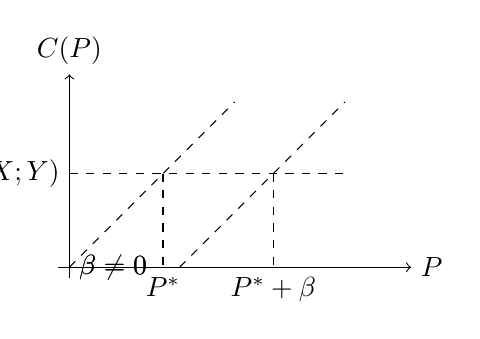
\begin{tikzpicture}[scale=0.7]
      % Grid
      %\draw[gridstyle] (-0.1,-0.1) grid (6.1,4.1);

      % Axes
      \draw[->] (-0.2,0) -- (6.2,0) node[right] {$P$};
      \draw[->] (0,-0.2) -- (0,3.5) node[above] {$C(P)$};

      % Tangents
      \draw[black,dashed] (0,0) -- (3,3);
      \draw[black,dashed] (2,0) -- (5,3);

      % First function
      \draw[color=black,domain=0.5:3.5] plot[id=cp1]
      function{1.5 * log(1 + (x-0.5)) / log(2)} node[right] {$\beta = 0$};

      % Second function
      \draw[color=black,domain=2.5:5.5] plot[id=cp2]
      function{1.5 * log(1 + (x - 2.5)) / log(2)} node[right] {$\beta \ne 0$};

      % Label for mutual information
      \draw[dashed] (0,1.7) -- (5,1.7);
      \draw (0,1.7) node[left] {\hskip-1cm\mbox{$I(X;Y)$}};

      % Labels for costs.
      \draw[dashed] (1.7,1.7) -- (1.7,0) node[below] {$P^*$};
      \draw[dashed] (3.7,1.7) -- (3.7,0) node[below] {$P^* + \beta$};


    \end{tikzpicture}
  \end{center}
  \caption{A geometric interpretation of the proof of
  Proposition~\ref{prop:cucconverse}. A nonzero $\beta$ shifts the capacity-cost
  curve such that the tangent at the operating point no longer goes through the
  origin.}
  \label{fig:cuccongeom}
\end{figure}

Propositions~\ref{prop:ratepercost} and~\ref{prop:cucconverse} are summarized
in the following theorem. 

\begin{theorem}
  \label{thm:cuccond}
  Under the technical condition of Proposition~\ref{prop:cucconverse}, the
  channel input distribution~$\px$ achieves the capacity per unit cost of the
  DMC~$\pyx$ if and only if the cost function satisfies
  \begin{equation}
    \label{eq:optcostthm}
    \rho(x) = c \DD, \quad c > 0. 
  \end{equation}
  For continuous alphabets, the condition is sufficient but not necessary.
\end{theorem}

\begin{remark}
  \label{rem:tcontc1}
  This result is very much related to the following result~\cite[Section~2.3,
  Problem~2]{CsiszarK1981},~\cite{GastparRV2003}. The channel input
  distribution $\px$ achieves the capacity of the channel $\pyx$ at expected
  cost $\E[\rho(X)]$ if and only if
  \[ \rho(x) = c(\DD + \beta) \]
  for some constants $c > 0$ and $\beta \in \R$. Our result shows that the extra
  requirement that capacity per unit cost be achieved restricts the possible
  cost functions to those with $\beta = 0$.
\end{remark}


\section{A Dual Result for the Source Coding Problem}
\label{sec:rddual}

Consider a discrete memoryless source (DMS) $S$ with distribution~$\ps$.
Let $V(\sh|s)$ and $W(\sh|s)$ be two test channels for the given source. 
Let $\psh$ and $\qsh$ be the
corresponding unconditional distributions of~$\Sh$, \ie,
\begin{align*}
  \psh(\sh) &= \sum_s \ps(s) V(\sh|s) \quad\text{and} \\
  \qsh(\sh) &= \sum_s \ps(s) W(\sh|s).
\end{align*}
Let $\dz$ be defined through $V(\sh|s)$ as follows:
\begin{equation}
  \label{eq:optimaldist}
   \dz(s, \sh) = -\log_2 \frac{V(\sh|s)}{\psh(\sh)} + \gamma(s),
 \end{equation}
 where $\gamma(s)$ is an arbitrary function of~$s$ satisfying $\E[\gamma(S)] =
 0$. 
Let $\Ev$ and $\Ew$ denote expectations over $S$ and~$\Sh$ with respect to $V$
and $W$, respectively, and let $\Iv(S;\Sh)$ and $\Iw(S;\Sh)$ be the
corresponding mutual informations. 

\begin{proposition}
  \label{prop:rateperdist}
  \begin{equation}
    \label{eq:rateperdist}
    \frac{\Ew[\dz(S,\Sh)]}{\Iw(S;\Sh)} \ge \frac{\Ev[\dz(S,\Sh)]}{\Iv(S;\Sh)} =
    -1,
  \end{equation}
  with equality if and only if $V(\sh|s) = W(\sh|s)$ for all~$s$ and~$\sh$.
\end{proposition}

Proposition~\ref{prop:rateperdist} implies that when the distortion measure is
as in~\eqref{eq:optimaldist} then $V(\sh|s)$ is the test channel that minimizes
the ratio of distortion per rate.

\begin{proof}
  First note that $\Ev[\dz(S,\Sh)] = -\Iv(S;\Sh)$, \ie,
  $\Ev[\dz(S,\Sh)]/\Iv(S;\Sh) = -1$. Next,
  \begin{align*}
    \lefteqn{\Iw(S;\Sh) + \Ew[\dz(S,\Sh)]} \\
    &=
    \sum_{s,\sh} \ps(s)W(\sh|s) \left[ \log_2 \frac{W(\sh|s)}{\qsh(\sh)} -
    \log_2 \frac{V(\sh|s)}{\psh(\sh)} \right] \\
    &= \sum_{s,\sh} \ps(s)W(\sh|s) \left[ \log_2\frac{W(\sh|s)}{V(\sh|s)} -
    \log_2 \frac{\qsh(\sh)}{\psh(\sh)} \right] \\
    &= \sum_s \ps(s) D(W(\cdot|s) \| V(\cdot |s)) - D(\qsh(\sh) \| \psh(\sh)) \\
    &\ge 0,
  \end{align*}
  where the inequality follows from the convexity of the Kullback-Leibler
  divergence (see \eg~\cite[Thm~2.7.2]{CoverT1991}); it becomes an equality iff
  $V(\sh|s) = W(\sh|s)$. Rearranging the inequality, we obtain
  \[ \frac{\Ew[\dz(S,\Sh)]}{\Iw(S;\Sh)} \ge -1. \]
\end{proof}


\begin{remark}
  This proposition holds also for continuous alphabets; just replace the
  sums in the proof by integrals.
\end{remark}

The distortion as defined in (\ref{eq:optimaldist}) may take positive and
negative values. In fact, Proposition~\ref{prop:rateperdist} shows that the
smallest achievable distortion per rate is $-1$.  The reader may find this
awkward; indeed it is hard to imagine an application where one would define a
distortion this way. The issue disappears if we define a {\em fidelity measure}
$\phi_0(s,\sh)=- \dz(s, \sh)$ and ask for the largest possible $\Ew[\po(S,\Sh)]
/ \Iw(S;\Sh)$, which will of course be $1$. Hence, for the rest of the paper we
will work with the the notion of fidelity, defined as the negative of the
distortion.\footnote{Of course mathematically the two notions are
quivalent.}

For later reference we restate Proposition~\ref{prop:rateperdist} in terms of
fidelity:

\begin{proposition}
  If $\po(s,\sh) = -\dz(s,\sh)$, then
  \label{prop:rateperfid}
  \begin{equation}
    \label{eq:rateperfid}
    \frac{\Ew[\phi_0(S,\Sh)]}{\Iw(S;\Sh)} \leq
    \frac{\Ev[\phi_0(S,\Sh)]}{\Iv(S;\Sh)} = 1,
  \end{equation}
  with equality if and only if $V(\sh|s) = W(\sh|s)$ for all~$s$ and~$\sh$.
\end{proposition}

Hence, if the fidelity measure is~$\po(s,\sh)$ then $V(\sh|s)$ is the test
channel that maximizes the \emph{fidelity per rate} of the source.

Analog to the rate-distortion function we can define 
\[ R(\Phi) = \min_{p(\sh|s): \E[\phi(S,\Sh)] \ge \Phi} I(S;\Sh) \]
as the \emph{rate-fidelity function} of the source at average fidelity~$\Phi$.
The rate-fidelity function has the same operational meaning as the
rate-distortion function: for each rate larger than $R(\Phi)$ there exists a
source code that achieves fidelity~$\Phi$, and
conversely no such code exists with a rate smaller than~$R(\Phi)$.


%\begin{example}[Binary]
%  \label{ex:bssrd}
%  Consider a transmission of a binary symmetric source with distribution $\ps(0)
%  = 1-p$, $\ps(1) = p$ across a binary symmetric channel of crossover
%  probability~$\e$. Let the encoder/decoder be the identity maps, \ie, $X = S$
%  and $\Sh = Y$. The conditional distribution~$V(\sh|s)$ is given by the matrix
%  \[ \left[
%  \begin{array}{cc}
%    1-\e & \e \\
%    \e & 1-\e
%  \end{array}
%  \right]
%  \]
%  and the distribution of~$\Sh$ is
%  \begin{align*}
%    \psh(0) &= (1-\e)(1-p) + \e p \\
%    \psh(1) &= \e(1-p) + (1-\e) p.
%  \end{align*}
%  Evaluating~\eqref{eq:optimaldist} for $p = 0.3$, $\e = 0.1$ results in
%  \begin{align*}
%    \dz(0,0) &\approx -0.45 & \dz(1,0) &\approx 2.72  \\
%    \dz(0,1) &\approx 1.77 & \dz(1,1) &\approx -1.404.
%  \end{align*}
%  The average distortion is $\E[\dz(S,\Sh)] \approx -0.46$ and the mutual
%  information is $I(S;\Sh) \approx 0.46$, and indeed 
%  $\E[\dz(S,\Sh)]/I(S;\Sh) = -1$.
%\end{example}

\begin{example}[Gaussian]
  \label{ex:gaussfid2}
  Consider a memoryless Gaussian source~$S$ with zero mean and unit variance,
  and a test channel $V(\sh|s)$ such that $\Sh$ given $S=s$ is distributed
  as\footnote{We use $\N(\mu, \sigma^2)$ to denote a Gaussian distribution of
  mean~$\mu$ and variance~$\sigma^2$.}
  \[ \N\left( \frac{\alpha}{\alpha+1}s, \frac{ \alpha}{(\alpha+1)^2}
  \right) \]
  for some $\alpha > 0$. Then $\Sh$ is distributed as $\N(0, \alpha /
  (\alpha + 1))$, and~$\po(s,\sh)$ evaluates to
  \begin{align*}
    \log_2 \frac{V(\sh|s)}{\psh(\sh)} 
%    &= \log_2 (P+1) + \frac{s^2}{2\ln 2 \ssq} - \frac{P + 1}{2 \ln 2\ssq}(s -
%    \sh)^2 \\
    &= c \left( k_1 + k_2 s^2 -(s-\sh)^2 \right)
  \end{align*}
  for some postive constants $c$, $k_1$, and $k_2$.
  
  The rate-fidelity function corresponding to~$\po(s,\sh)$ is
  \begin{equation*}
    R(\Phi) = \frac{1}{2} \log_2 \frac{\ssq}{k_1 + k_2 \ssq - \Phi/c}.
  \end{equation*}
  The plot of $\Phi$ vs.\ $R(\Phi)$ on Figure~\ref{fig:ratefidplot} bears a
  strong resemblance to~Figure~\ref{fig:gausscap}: a tangent of slope~$1$
  touches the curve in the operating point corresponding to $\ps$
  and~$V(\sh|s)$. 
  \begin{figure}
    \begin{center}
      \begin{tikzpicture}[scale=0.6]
        \draw[gridstyle] (-0.1,-0,1) grid (6.1,4.1);

        % Axes
        \draw[->] (-0.1,0) -- (6.2,0) node[right] {$R(\Phi)$};
        \draw[->] (0,-2.8) -- (0, 2.8) node[above] {$\Phi$};

        \draw[dashed] (0,1.4) node[left] {$\E[\phi(S,\Sh)]$} -- (1.6,1.4);
        \draw[dashed] (1.4,0) -- (1.4,1.6);
        \node at (1.6,0) [below] {$I(S;\Sh)$};


        % The function to plot
        \draw[color=black,domain=0:5.5] plot[id=rfid] 
        function{19*(0.1 + 0.01 - 2**(-2*(x+1)))};
        \draw[color=red,domain=0:2.5] plot[id=tangent2]
        function{x};
      \end{tikzpicture}
    \end{center}
    \caption{Average fidelity~$\Phi$ vs.\ minimum rate~$R(\Phi)$ for
    Example~\ref{ex:gaussfid2}. The similarity to Figure~\ref{fig:gausscap}
    illustrates that the fidelity per rate is to a source what the capacity per
    cost is to a channel.}
    \label{fig:ratefidplot}
  \end{figure}
\end{example}

Does the fidelity obtained in the above example make sense? The multiplicative
constant $c$ is unavoidable: it accounts for the fact that one is free to choose
the units. The term $k_2s^2-(s-\sh)^2$ indicates that the tolerance for the
error $(s-\sh)^2$ is relative to $s^2$. In other words, small errors when $s^2$
is small are considered at the same level of satisfaction as large errors when
$s^2$ is large, provided that $k_2s^2-(s-\sh)^2$ is constant. Finally, the
constant $k_1$ accounts for the fact that the degree of satisfaction at the same
value of $k_2s^2-(s-\sh)^2$ may vary from one application to another: a
radiologist looking at an x-ray will have a smaller error tolerance than a
person listening to music in a noisy environment.

The next proposition says that the fidelity measure~$\phi(s,\sh)$ for which a
given test channel maximizes the fidelity per rate is unique up to addition of a
function of~$s$ with zero mean.

\begin{proposition}
  \label{prop:rdconverse}
  Let $\ps$ be a discrete memoryless source with fidelity measure~$\phi(s,\sh)$
  and rate-fidelity function~$R(\Phi)$. If the test channel $V(\sh|s)$ maximizes
  the ratio
  \[ \frac{\E[\phi(S,\Sh)]}{I(S;\Sh)} \]
  among all test channels and if the derivative of~$R(\Phi)$ exists at $\Phi =
  \Ev[\phi(S,\Sh)]$, then $\phi(s,\sh) = c \po(s,\sh)$ for some $c > 0$.
\end{proposition}

The proof mimics that for Proposition~\ref{prop:cucconverse}. In particular,
after taking expectation over~$S$ the function~$\gamma(s)$ becomes a constant
that plays the same role that $\beta$ plays in the proof of
Proposition~\ref{prop:cucconverse}.
%\begin{remark}
%  \label{rem:rdderivative}
%  The authors do not know whether there are sources\slash distortion measures
%  for which the rate-distortion function is not differentiable. It might be that
%  the technical conditions of Propositions~\ref{prop:cucconverse}
%  and~\ref{prop:rdconverse} are always satisfied.
%\end{remark}

Propositions~\ref{prop:rateperfid} and~\ref{prop:rdconverse} are summarized in
the following theorem.
\begin{theorem}
  \label{thm:rdthm}
  Under the technical condition of Proposition~\ref{prop:rdconverse}, the
  test channel~$V(\sh|s)$ maximizes the fidelity per rate of a
  discrete memoryless source if and only if the fidelity measure satisfies
  \begin{equation}
    \label{eq:optfid}
    \phi(s,\sh) = c \log_2\frac{V(\sh|S)}{\psh} + \gamma(s), \quad c > 0
  \end{equation}
  with $\E[\gamma(S)] = 0$.  For continous sources, the condition is sufficient
  but not necessary.
\end{theorem}

\begin{remark}
  \label{rem:tcontc2}
  This result is very much related to the following result~\cite[Section~2.3,
  Problem~3]{CsiszarK1981},~\cite{GastparRV2003} (restated here in terms of
  fidelity). The test channel $V(\sh|s)$
  achieves the rate-fidelity function of the source $\ps$ at expected
  fidelity $\E[\phi(S,\Sh)]$ if and only if
  \[ \phi(s,\sh) = c \log_2 \frac{V(\sh|s)}{\psh} + \gamma(s) \]
  for $c > 0$ and an arbitrary function $\gamma(s)$. Our result shows that the
  extra requirement that the maximum fidelity per rate be achieved restricts the
  allowed fidelity functions to those with $\E[\gamma(S)] = 0$.
\end{remark}


%In this context, we can interpret bits as a kind of currency that we pay to
%get a certain fidelity; to use the available bits (e.g. disk space, rate of a
%channel) most efficiently, one would like to get the most fidelity per bit.

In analogy to the capacity per unit cost we define the \emph{fidelity per unit
rate} of a discrete memoryless source as
\[ \Phih = \sup_{V(\sh|s)} \frac{\Ev[\phi(S,\Sh)]}{\Iv(S;\Sh)} =  \sup_{\Phi}
\frac{\Phi}{R(\Phi)}. \]
In light of the previous observations, this quantity is to the source what the
capacity per unit cost is to the channel. 

\begin{remark}\label{rem:verduphi}
  To establish a connection with the perspective offered in Section~IV of
  Verd\'u's paper~\cite{Verdu1990}, let $\Phi_0$ be the maximum fidelity that
  can be achieved when representing the source by a fixed symbol, \ie, $\Phi_0 =
  \max_{\sh} \E[\phi(S, \sh)]$. The following applies:
\begin{itemize}
  \item If $\Phi_0 > 0$ then $\Phih = \infty$. Indeed, the positive
    fidelity~$\Phi_0$ is achieved at zero rate.
  \item If $\Phi_0 < 0$ then $0 < \Phih < \infty$. 
  \item If $\Phi_0 = 0$ then $\Phih = \lim_{\Phi \searrow 0} \Phi /
    R(\Phi)$. 
\end{itemize}
The three cases are illustrated in \figref{verduphi}.

This differs from Verd\'u's approach in that the latter -- if stated in terms of
fidelity -- defines the counterpart to the capacity per unit cost to be
$\lim_{\Phi \searrow \Phi_0} \Phi / R(\Phi)$ regardless of the value
of~$\Phi_0$. 
\end{remark}

\begin{figure}
  {
\newcommand{\clipcmd}{\path[clip] (-1.25,-1) rectangle (3.2,3.5);}
\newcommand{\myaxes}{
        \draw[->] (-0.1,0) -- (2.2,0) node[right] {$R(\Phi)$};
        \draw[->] (0,-2.8) -- (0, 2.8) node[above] {$\Phi$};
}

\subfloat[$\Phi_0 > 0$]{
      \begin{tikzpicture}[baseline=0pt,font=\scriptsize]
        \clipcmd

        % Axes
        \myaxes

        % The function to plot
        %%%% First version, \Phi > 0 %%%%%
        \begin{scope}[yshift=3.5cm]
          \draw[color=black,domain=0:.75] plot[id=rfid2_short] 
          function{19*(0.1 + 0.01 - 2**(-2*(x+1)))};
          \draw[dashed] (0,-2.66) -- (-.5,-2.66) node [left] {$\Phi_0$};
        \end{scope}

        \draw[red] (0,0) -- (0,0.84);

        %%%% END \Phi > 0 %%%%%%

        \end{tikzpicture}}
      \hfil
      \subfloat[$\Phi_0 < 0$]{
      \begin{tikzpicture}[baseline=0pt,font=\scriptsize]
        \clipcmd

        % Axes
        \myaxes

        % The function to plot
        %%%% Second version, \Phi < 0 %%%%
          \draw[color=black,domain=0:3] plot[id=rfid2] 
          function{19*(0.1 + 0.01 - 2**(-2*(x+1)))};
          \draw[color=red,domain=0:2.5] plot[id=tangent2]
          function{x};

          \draw[dashed] (0,-2.66) -- (-.5,-2.66) node [left] {$\Phi_0$};
        %%%% END \Phi < 0 %%%%
        
        % A label with an arrow for \Phi_0.
        \node (phizlabel) at (-0.75,-0.25) {$\Phi_0$};
        \draw[->] (phizlabel) -- +(.25,-.5);

      \end{tikzpicture}}
      \hfil
      \subfloat[$\Phi_0 = 0$]{
      \begin{tikzpicture}[baseline=0pt,font=\scriptsize]
        \clipcmd

        % Axes
        \myaxes

        % The function to plot
        %%%% Third version, \Phi = 0 %%%%
        \begin{scope}[yshift=2.66cm]
          \draw[color=black,domain=0:1] plot[id=rfid2_short2] 
          function{19*(0.1 + 0.01 - 2**(-2*(x+1)))};
          \draw[dashed] (0,-2.66) -- (-.5,-2.66) node [left] {$\Phi_0$};
        \end{scope}

        \draw[red] (0,0) -- (.5,3);

        %%%% End Third version

      \end{tikzpicture}
      }
      }
      \caption{The three possible cases for $\Phi_0$ as discussed in
      \remref{verduphi}.}
  \label{fig:verduphi}
\end{figure}


\section{Fidelity Per Unit Cost}
\label{sec:fidcostbound}

The problems considered in the two previous sections are instances of a general
class of problems where resources are traded against performance.  In the
channel case, we spend a cost (the resource) to achieve a high rate
(the performance), and we want to maximize the
performance per unit of resource. In the source case, we spend bits (the
resource) to achieve a high fidelity (the performance), and once again we want
to maximize the performance per unit of resource.  

In this section we consider the end-to-end communication problem, where the
resource is the channel input cost and the performance is the fidelity of the
source reproduction. The goal is to maximize the \emph{fidelity per cost}. The
aim of this section is to find a tight bound on this ratio and  to characterize
the operating point that achieves the bound.

From the separation theorem, the average fidelity and cost of any communication
system must satisfy
\begin{equation}
  \label{eq:sepineq}
  k R(\Phi) \le n C(P),
\end{equation}
where $k$ and $n$ are the number of source symbols and channel uses per time,
respectively. Furthermore, the largest achievable $\Phi$ for a fixed~$P$ is the
one for which the above inequality is satisfied with equality.
Conversely, any fidelity/cost pair satisfying the inequality can
be approached by a suitable communication system using separate source and
channel coding.

Using the definitions of $\Phih$ and $\Ch$,
\begin{align*}
  \Phih &= \sup_\Phi \frac{\Phi}{R(\Phi)} & \Ch &= \sup_P \frac{C(P)}{P},
\end{align*}
together with~\eqref{eq:sepineq}, we obtain the following tight bound on the
fidelity per cost:
\begin{equation}
  \label{eq:extineq}
\frac\Phi P = \frac\Phi{R(\Phi)} \cdot \frac{R(\Phi)}{C(P)} \cdot
\frac{C(P)}{P} \le \frac nk \Ch \Phih.
\end{equation}
We call the right-hand side of~$\eqref{eq:extineq}$ the \emph{fidelity per unit
cost} of the communication system.

A separation-based communication system achieves the fidelity per unit cost if
and only if 
\begin{enumerate}
\item the source encoder and decoder operate at $\Phih,$
\item the channel encoder and decoder operate at $\Ch$, and
\item the number of bits produced by the source encoder for $k$ source symbols
  equals the number of bits transmitted on the channel in $n$ channel uses. 
\end{enumerate}


Using the converse to the source-channel coding theorem as done
in~\cite{GastparThesis} along with the results of the previous two
sections we
can translate the conditions for equality in~\eqref{eq:extineq} into conditions
that apply to any system that achieves the maximum fidelity per cost, regardless
of whether the system relies on the separation principle, on joint
source-channel block coding, or on uncoded communication.  These general
conditions are stated in the following theorem.


\begin{theorem}
  \label{thm:bla}
  A discrete point-to-point communication system of the type shown in
  Figure~\ref{fig:scmodel} achieves the fidelity per unit cost if and only if
  all of the following conditions are satisfied.

\begin{enumerate}
  \item The reproduction is related to the source via the test channel, \ie,
    \[P_{\Sh^k|S^k}(\sh^k|s^k)=\prod_{i=1}^k
    V(\sh_i|s_i), \]
    where $s^k =(s_1, \ldots, s_k)$     and where $V$ relates to the fidelity
    function according to~\eqref{eq:optfid}.
  \item The channel input is \iid\ with distribution $P_X$ that achieves
    capacity per unit cost, \ie, it relates to the cost function according
    to~\eqref{eq:optcostthm}.
  \item The encoder and decoder are information lossless in the sense that
    $kI(S;\Sh) = n I(X;Y)$.  
\end{enumerate}
\end{theorem}

\begin{figure}
  \begin{center}
    \begin{tikzpicture}[node distance=2.5cm]
      \node[sc] (source) at (0,0)  {\textsc{dms}};
      \node[c] (enc) [right of=source] {encoder};
      \node[sc] (channel) [right of=enc] {\textsc{dmc}};
      \node[c] (dec) [right of=channel] {decoder};
      \node[sc] (rec) [right of=dec] {receiver};
      
      % Connections between source, channel, etc.
      \draw[l] (source) -- node[above] {$S^k$} (enc);
      \draw[l] (enc) -- node[above] {$X^n$} (channel);
      \draw[l] (channel) -- node [above] {$Y^n$} (dec);
      \draw[l] (dec) -- node[above] {$\hat S^k$} (rec);
    \end{tikzpicture}

  \end{center}
  \caption{A point-to-point communication system consisting of a discrete
  memoryless source (DMS) with distribution~$\ps$, a discrete memoryless channel
  (DMC) with transition probabilities~$\pyx$, an encoder and a decoder.}
  \label{fig:scmodel}
\end{figure}

This result is a refinement of \thmref{optimalityconditions}, which gave
necessary and sufficient conditions for the cost~$P$ and distortion~$D$ of a
point-to-point communication system to satisfy $k R(D) = n C(P)$. According
to~\eqref{eq:extineq}, a communication system that operates at fidelity per unit
cost also satisfies $k R(D) = n C(P)$, so it is also optimal in the sense of
\defref{optimality}.
